%%%%%%%%%%%%%%%%%%%%%%%%%%%%%%%%%%%%%%%%%%%%%%%%%%%%%%%%%%%%%%%%%%%%%%%%%%%%%%%%%%%
%% This project aims to create the UFC template for presentation.                %%
%% author: Maurício Moreira Neto - Doctoral student in Computer Science (MDCC)   %%
%% contacts:                                                                     %%
%%    e-mail: maumneto@ufc.br                                                    %%
%%    linktree: https://linktr.ee/maumneto                                       %%
%%%%%%%%%%%%%%%%%%%%%%%%%%%%%%%%%%%%%%%%%%%%%%%%%%%%%%%%%%%%%%%%%%%%%%%%%%%%%%%%%%%
\documentclass{libs/SUSTech_format}
\usepackage{ctex}
\usepackage{tipa}
\usepackage{unicode-math}
\usepackage{amsmath}
\graphicspath{{fig/}}

\def\cmd#1{\texttt{\color{DarkBlue}\footnotesize $\backslash$#1}}
\def\env#1{\texttt{\color{DarkBlue}\footnotesize #1}}
\def\cmdxmp#1#2#3{\small{\texttt{\color{DarkBlue}$\backslash$#1}\{#2\}\hspace{1em}\\ $\Rightarrow$\hspace{1em} {#3}\par\vskip1em}}
\newcommand\pkg[1]{\texttt{#1}}

% Inserting the preamble file with the packages
%%%%%%%%%%%%%%%%%%%%%%%%%%%%%%%%%%%%%%%%%%%%%%%%%%%%%%%%%%%%%%%%%%%%%
%% This file contains the packages that can be used in the beamer. %%
%%%%%%%%%%%%%%%%%%%%%%%%%%%%%%%%%%%%%%%%%%%%%%%%%%%%%%%%%%%%%%%%%%%%%
% Package to fonts family
\usepackage[T1]{fontenc}
% Package to accentuation
\usepackage[utf8]{inputenc}
% Package to Portuguese language
\usepackage[english]{babel}
% Package to Figures
\usepackage{graphicx}
% Package to the colors
\usepackage{color}
% Package to the colors
\usepackage{xcolor}
% Packages to math symbols and expressions
\usepackage{amsfonts, amssymb, amsmath}
% Package to multiple lines and columns in table
\usepackage{multirow, array} 
% Package to create pseudo-code
% For more detail of this package: http://linorg.usp.br/CTAN/macros/latex/contrib/algorithm2e/doc/algorithm2e.pdf
\usepackage{algorithm2e}
% Package to insert code
\usepackage{listings} 
\usepackage{keyval}
% Package to justify text
\usepackage[document]{ragged2e}
% Package to manage the bibliography
\usepackage[backend=biber, style=numeric, sorting=none]{biblatex}
% Package to facilities quotations
\usepackage{csquotes}
% Package to use multicols
\usepackage{multicol}
\usepackage{minted}

% Inserting the references file
\bibliography{references.bib}

\usefonttheme{serif,professionalfonts}

% Title
\title[\LaTeX 入门]{\huge \textbf{\LaTeX 入门}}
% Subtitle
% \subtitle{Subtitle of the Presentation}
% Author of the presentation
\author{李子强 \hspace{0.5em}计算机系}
% Institute's Name
\institute[SUSTech]{
    % email for contact
    % \normalsize{\email{lizq2019@mail.sustech.edu.cn}}
    % \newline
    % Department Name
    % \department{Name of the Department}
    % \newline
    % university name
    % \SUSTech
    \normalsize
    南方科技大学
}
% date of the presentation
\date{2021年3月31日}




%%%%%%%%%%%%%%%%%%%%%%%%%%%%%%%%%%%%%%%%%%%%%%%%%%%%%%%%%%%%%%%%%%%%%%%%%%%%%%%%%%
%% Start Document of the Presentation                                           %%               
%%%%%%%%%%%%%%%%%%%%%%%%%%%%%%%%%%%%%%%%%%%%%%%%%%%%%%%%%%%%%%%%%%%%%%%%%%%%%%%%%%
\begin{document}
% insert the code style
%%%%%%%%%%%%%%%%%%%%%%%%%%%%%%%%%%%%%%%%%%%%%%%%%%%%%%%%%%%%%%%%%%%%%%%%%%%%%%%%%%%
%% This file contains the style of the codes show in slides.                     %%
%% The package used is listings, but it possible to used others.                 %%
%%%%%%%%%%%%%%%%%%%%%%%%%%%%%%%%%%%%%%%%%%%%%%%%%%%%%%%%%%%%%%%%%%%%%%%%%%%%%%%%%%%

% color used in the code style
\definecolor{codegreen}{rgb}{0,0.6,0}
\definecolor{codegray}{rgb}{0.5,0.5,0.5}
\definecolor{codepurple}{rgb}{0.58,0,0.82}
\definecolor{codebackground}{rgb}{0.95,0.95,0.92}

% style of the code!
\lstdefinestyle{codestyle}{
    backgroundcolor=\color{codebackground},   
    commentstyle=\color{codegreen},
    keywordstyle=\color{magenta},
    numberstyle=\tiny\color{codegray},
    stringstyle=\color{codepurple},
    basicstyle=\ttfamily\footnotesize,
    frame=single,
    breakatwhitespace=false,         
    breaklines=true,                 
    captionpos=b,                    
    keepspaces=true,                 
    numbers=left,                    
    numbersep=4pt,                  
    showspaces=false,                
    showstringspaces=false,
    showtabs=false,                  
    tabsize=2,
    title=\lstname 
}

\lstset{style=codestyle}

% Style of Algrithm



% Style of minted


%% ---------------------------------------------------------------------------
% First frame (with tile, subtitle, ...)
% \begin{frame}{}
%     %% Putting the background image in the frames
%     \usebackgroundtemplate{
\includegraphics[width=1.7\paperwidth]{libs/LOGO transparent.png}}
%     \maketitle
% \end{frame}

{
    \usebackgroundtemplate{
\includegraphics[width=1.7\paperwidth]{libs/LOGO transparent.png}}
    \begin{frame}
    \maketitle
    \end{frame}
}

%% ---------------------------------------------------------------------------
% Second frame
\begin{frame}{目录}
    \begin{multicols}{2}
        \tableofcontents
    \end{multicols}
\end{frame}


%% ---------------------------------------------------------------------------
% This presentation is separated by sections and subsections

\section{介绍}

\subsection{\TeX 排版系统历史}

\begin{frame}[fragile]{\TeX 与 \LaTeX 的起源}
  \begin{columns}[T]
    \column{.8\textwidth}
    \begin{itemize}
      \item \TeX: $\tau\varepsilon\chi$ (\textipa{/'tEx/},
        \textipa{/'tEk/})
        \begin{itemize}
          \item 生成精美图书的排版系统
          \item 最初由 高德纳 (Donald E.~Knuth) 于 1978 年开发
          \item 最新版本为 \TeX\ 3.14159265
          \item 漂亮、美观、稳定、通用
          \item 尤其擅长数学公式排版
        \end{itemize}

        \vspace{2em}
      \item \LaTeX\ (\textipa{/'la:tEx/}, \textipa{/'leItEk/})
        \begin{itemize}
          \item Leslie Lamport 开发的一种 \TeX 格式
          \item 在 \TeX 的基础上提供宏包, 降低使用门槛
          \item 极其丰富的宏包,提供扩展功能
          \item 广泛用于学术界,期刊会议论文模板
        \end{itemize}
    \end{itemize}
    \column{.2\textwidth}
    % \vspace*{5mm}
    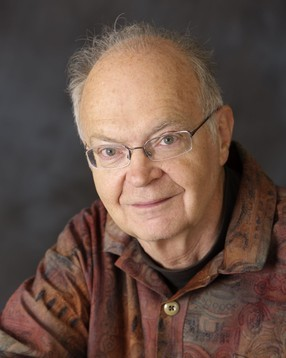
\includegraphics[width=\textwidth]{Knuth.jpg}

    % \vspace*{5mm}
    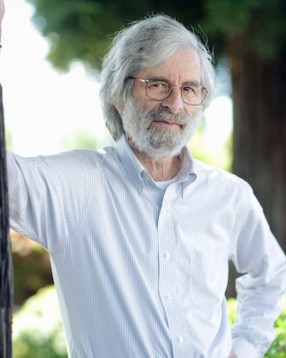
\includegraphics[width=\textwidth]{Lamport.jpg}

  \end{columns}
\end{frame}

\subsection{\LaTeX 利弊}

\begin{frame}[fragile]{\LaTeX 的好处与坏处}
    \textbf{好处}
    \begin{itemize}
        \item 数学公式排版优雅 \quad $\mathcal{F}(\xi)=\int_{-\infty}^{\infty} f(x)\mathrm{e}^{-\mathrm{j}2\pi \xi x}\,\mathrm{d}x$
        \item 内容与格式分离
        \item 随心所欲的宏定义与自定义命令 \rawcmd{\textbackslash newcommand},\rawcmd{\textbackslash def}
    \end{itemize}

    \vspace{2em}
    \textbf{坏处}
    \begin{itemize}
        \item 得到易读的版本,需要编译
        \item 输入相对 Word 繁琐
        \item 非开箱即用。有时自行解决编辑器、宏包,甚至是编译错误。
    \end{itemize}

\end{frame}

\subsection{本地安装,还是在线编辑?}

\begin{frame}[fragile]{选择发行版 -> 下载 -> 安装}
  \begin{itemize}
    \item Windows or Linux -> \texlive
      \begin{itemize}
        \item 下载 \texlive 离线安装镜像,每年 4月发布当年版本 \url{https://mirrors.sustech.edu.cn/CTAN/systems/texlive/Images/texlive.iso}
        \item 解压或挂载下载的 ISO,运行 \rawcmd{install-tl-windows.bat} (Windows) or \rawcmd{install-tl} (Linux)
        \item 切换默认仓库为国内镜像可加速今后升级
      \end{itemize}
    \item macOS -> \mactex
      \begin{itemize}
        \item $\approx$ \texlive 在 Mac 下重新封装版本
        \item 需要下载独立的安装包 \url{https://mirrors.sustech.edu.cn/CTAN/systems/mac/mactex/MacTeX.pkg}
      \end{itemize}
\end{itemize}
    \emph{不推荐安装 C\TeX 套装}
    \begin{itemize}
        \item \emph{存在严重 bug,并且完全过时(2012年已经停止维护)。}
    \end{itemize}
\end{frame}

\begin{frame}[fragile]{选择本地编辑器}
  \begin{itemize}
    \item<+-> 专用型
  
      \begin{itemize}
        \item TeXworks:\TeX{} Live 自带 \faWindows{} \faApple{} \faLinux{}
        \item \emph{TeXstudio}:功能丰富,对新手友好 \faWindows{} \faApple{} \faLinux{}
        \item TeXShop:Mac\TeX{} 自带 \faApple{}
        \item WinEdt:功能丰富,收费 \faWindows{}
      \end{itemize}
  
    \item<+-> 通用型
  
      \begin{itemize}
        \item \emph{Visual Studio Code}:\pkg{LaTeX Workshop} (James Yu @ CSE) + \pkg{LaTeX Utilities}
        \item Atom:听说很卡?
        \item Sublime Text:收费
        \item Vim:|q|、|q!|、|wq|、|wq!|
      \end{itemize}

    \item<+-> 编辑器对比:\link{https://tex.stackexchange.com/q/339}
                          \link{https://en.wikipedia.org/wiki/Comparison_of_TeX_editors}
                          \link{https://www.zhihu.com/question/19954023}
  \end{itemize}
\end{frame}


\begin{frame}[fragile]{太麻烦!用在线的}

    \begin{itemize}
        \item 通过在线平台编辑、编译
        \item 免去安装/升级等一系列烦恼 可以多人协作 支持中文,但有时需要自己上传字体
        \item 可以多人协作
        \item 支持中文,但有时需要自己上传字体
    \end{itemize}

    \begin{itemize}
      \item Overleaf
      \begin{itemize}
          \item \url{https://www.overleaf.com}
      \end{itemize}
      \item ShareLaTex by 计算机研究协会
      \begin{itemize}
        \item \url{https://sharelatex.cra.moe/}
    \end{itemize}
      \end{itemize}
  \end{frame}

\section{填写创作}

\subsection{文件结构}

\begin{frame}[fragile]{文件结构}
    \lstset{language=[LaTeX]TeX}
    \begin{lstlisting}[basicstyle=\ttfamily]
  \documentclass[a4paper]{article}
  % 文档类型,如 article,[]内是选项,如 a4paper
  % 这里开始是导言区
  \usepackage{graphicx} % 引用宏包
  \graphicspath{{fig/}} % 设置图片目录
  % 导言区到此为止
  \begin{document}
  这里开始是正文
  \end{document}\end{lstlisting}
  \end{frame}

\subsection{常用命令}
  
\begin{frame}[fragile]{\LaTeX“命令”}
    \framesubtitle{\emph{宏} (Macro)、或者\emph{控制序列} (control sequence)}
  \begin{itemize}
  \item 简单命令
    \begin{itemize}
      \item \verb|\命令|\hspace{2em}
      \verb|{\songti 中国人民解放军}| ~$\Rightarrow$ {\songti 中国人民解放军}
    \item \verb|\命令[可选参数]{必选参数}|\\
  \verb|\section[精简标题]{这个题目实在太长了放到目录里面不太好看}|\\
  $\Rightarrow$ {\heiti 1.1 \hspace{1em} \songti 这个题目实在太长了放到目录里面不太好看}
    \end{itemize}
  \item 环境
    \begin{columns}[c]
    \begin{column}{0.45\textwidth}
      \begin{lstlisting}[basicstyle=\ttfamily]
  \begin{equation*}
    a^2-b^2=(a+b)(a-b)
  \end{equation*}\end{lstlisting}
  \end{column}\hspace{1em}
    \begin{column}{0.45\textwidth}
  $ a^2-b^2=(a+b)(a-b)$
  \end{column}
    \end{columns}
  \end{itemize}
  \end{frame}
  
  % \begin{frame}[fragile]{\LaTeX 常用命令}
  %   \begin{exampleblock}{简单命令}
  % \centering
  % \footnotesize
  %   \begin{tabular}{llll}
  %     \cmd{chapter} & \cmd{section} & \cmd{subsection} & \cmd{paragraph} \\
  %     章 & 节 & 小节 & 带题头段落 \\\hline
  %     \cmd{centering} & \cmd{emph} & \cmd{verb} & \cmd{url} \\
  %    居中对齐         &  强调      & 原样输出   & 超链接 \\\hline
  %   \cmd{footnote} & \cmd{item} & \cmd{caption} & \cmd{includegraphics} \\
  %    脚注 & 列表条目 & 标题 & 插入图片 \\\hline
  %   \cmd{label} & \cmd{cite} & \cmd{ref} \\
  %   标号 & 引用参考文献 & 引用图表公式等\\\hline
  %   \end{tabular}
  % \end{exampleblock}
  % \end{frame}
  \begin{frame}[fragile]{谋篇布局}
  \begin{itemize}
    \item 文档部件
  
      \begin{itemize}
        \item 标题:|\title|、|\author|、|\date| $\to$ |\maketitle|
        \item 摘要:|abstract| 环境
        \item 目录:|\tableofcontents|
        \item 章节:|\chapter|、|\section|、|\subsection| 等
        \item 图表:|\table|、|\figure|
        \item 引用:|\label|、|\cite|、|\ref|
        \item 文献:|\bibliography|
      \end{itemize}
  
    \item 文档划分
  
      \begin{itemize}
        \item 凤头猪肚豹尾:|\frontmatter|、|\mainmatter|、|\backmatter|
        \item 分文件编译:|\include|、|\input|
      \end{itemize}
  \end{itemize}
  \end{frame}

  \begin{frame}[fragile]
    \frametitle{文本标记}
    \begin{itemize}
      \item 加粗:|{\bfseries ...}| 或 |\textbf{...}|
      \item 倾斜:|{\itshape ...}| 或 |\textit{...}|
      \item 字号:|\tiny|、|\small|、|\large|、|\Large| 等
      \item 换行:|\\|
      \item 缩进:|\indent|
      \item 居中:|\centering| 或 |center| 环境
    \end{itemize}
  \end{frame}
    

  \begin{frame}{\LaTeX 命令举例}
    \cmdxmp{chapter}{前言}{\heiti 第 1 章\hspace{1em} 前言}
    \cmdxmp{section[精简标题]}{这个题目实在太长了放到目录里面不太好看}{\heiti 1.1
      \hspace{1em} 这个题目实在太长了放到目录里面不太好看}
    \cmdxmp{footnote}{我是可爱的脚注}{前方高能\footnote{我是可爱的脚注}}
    \end{frame}
    
  \subsection{环境}
  \begin{frame}[fragile]{\LaTeX 常用命令}
  \begin{exampleblock}{环境}
  \centering
  \footnotesize
  \begin{tabular}{lll}
    \env{table} & \env{figure} & \env{equation}\\
    表格 & 图片 & 公式 \\\hline
    \env{itemize} & \env{enumerate} & \env{description}\\
    无编号列表 & 编号列表 & 描述 \\\hline
  \end{tabular}
  \end{exampleblock}
  \end{frame}
  
\subsection{列表}
\begin{frame}[fragile]{\LaTeX 环境举例}
    \vspace{1em}
      \begin{minipage}{0.4\linewidth}
        \begin{lstlisting}[basicstyle=\ttfamily\small]
    \begin{itemize}
      \item 一条
      \item 次条
      \item 这一条可以分为 ...
        \begin{itemize}
          \item 子一条
        \end{itemize}
    \end{itemize}\end{lstlisting}
      \end{minipage}\hspace{1.5cm}
      \begin{minipage}{0.4\linewidth}
    \begin{itemize}
      \item 一条
      \item 次条
      \item 这一条可以分为 ...
        \begin{itemize}
          \item 子一条
        \end{itemize}
    \end{itemize}
      \end{minipage}
    % \smallskip
    
    \begin{minipage}{0.4\linewidth}
    \begin{lstlisting}
    \begin{enumerate}
      \item 一条
      \item 次条
      \item 再条
    \end{enumerate}\end{lstlisting}
      \end{minipage}\hspace{1.5cm}
      \begin{minipage}{0.4\linewidth}
        \vspace{-1cm}
    \begin{enumerate}
      \item 一条
      \item 次条
      \item 再条
    \end{enumerate}
      \end{minipage}
    \end{frame}
    %
    
  \begin{frame}[fragile]{列表与枚举}
    \begin{columns}
    \begin{column}{.6\textwidth}
    \begin{lstlisting}[basicstyle=\ttfamily\small]
    \begin{enumerate}
    \item \LaTeX 好处都有啥
      \begin{description}
        \item[好用] 体验好才是真的好
        \item[好看] 强迫症的福音
        \item[开源] 众人拾柴火焰高
      \end{description}
    \item 还有呢?
      \begin{itemize}
        \item 好处 1
        \item 好处 2
      \end{itemize}
    \end{enumerate}
    \end{lstlisting}
    \end{column}
    \begin{column}{.4\textwidth}
    {\small
    \begin{enumerate}
    \item \LaTeX 好处都有啥
      \begin{description}
        \item[好用] 体验好才是真的好
        \item[好看] 治疗强迫症
        \item[开源] 众人拾柴火焰高
      \end{description}
    \item 还有呢?
      \begin{itemize}
        \item 好处 1
        \item 好处 2
      \end{itemize}
    \end{enumerate}
    }
    \end{column}
    \end{columns}
    
    \end{frame}
    


    \subsection{数学公式}
    \begin{frame}[fragile]{\LaTeX 数学公式}
        \begin{itemize}
        \item 数学公式排版是 \LaTeX 的绝对强项
        \item 数学排版需要进入数学模式,引用 \texttt{amsmath} 宏包
            \begin{itemize}
            \item 用单个美元符号(\verb|$|) 包围起来的内容是 {\bf 行内公式}
          \item 用两个美元符号(\verb|$$|) (不推荐)或 \verb|\[ \]| 包围起来的是 {\bf 单行公式} 或 {\bf 行间公式}
            \item 使用数学环境,例如 \texttt{equation} 环境内的公式会自动加上编号,
                \texttt{align} 环境用于多行公式(例如方程组、多个并列条件等)
          \end{itemize}
        \item 寻找符号
            \begin{itemize}
              \item 运行 \texttt{texdoc symbols} 查看符号表
              \item S. Pakin. \emph{The Comprehensive \LaTeX Symbol List}
                    \url{https://ctan.org/pkg/comprehensive}
              \item 手写识别(有趣但不全):Detexify \url{http://detexify.kirelabs.org}
            \end{itemize}
        \item MathType 也可以使用和导出 \LaTeX 公式(不推荐)
        \end{itemize}
        \end{frame}
    
        
    \begin{frame}[fragile]{\LaTeX 数学公式}
    
    \begin{columns}
    \begin{column}{.5\textwidth}
    \lstset{language=[LaTeX]TeX}
    \begin{lstlisting}[basicstyle=\ttfamily\small]
    $V = \frac{4}{3}\pi r^3$
    
    \[
      V = \frac{4}{3}\pi r^3
    \]
    
    \begin{equation}
    \label{eq:vsphere}
    V = \frac{4}{3}\pi r^3
    \end{equation}
    \end{lstlisting}
    \end{column}
    
    \begin{column}{.5\textwidth}
    $V = \frac{4}{3}\pi r^3$
    
    \[
      V = \frac{4}{3}\pi r^3
    \]
    
    \begin{equation}
    \label{eq:vsphere}
    V = \frac{4}{3}\pi r^3
    \end{equation}
    \end{column}
    \end{columns}
    
    \end{frame}

    
    \subsection{目录}
    \begin{frame}[fragile]{层次与目录生成}
    \begin{columns}
    \begin{column}{.6\textwidth}
    \lstset{language=[LaTeX]TeX}
    \begin{lstlisting}[basicstyle=\ttfamily\small]
    \tableofcontents % 这里是目录
    \part{有监督学习}
    \chapter{支持向量机}
    \section{支持向量机简介}
    \subsection{支持向量机的历史}
    \subsubsection{支持向量机的诞生}
    \paragraph{一些趣闻}
    \subparagraph{第一个趣闻}
    \end{lstlisting}
    \end{column}
    \begin{column}{.4\textwidth}
    第一部分\quad 有监督学习\\
    第一章\quad 支持向量机 \\
    1. 支持向量机简介 \\
    1.1 支持向量机的历史 \\
    1.1.1 支持向量机的诞生 \\
    一些趣闻  \\
    第一个趣闻
    \end{column}
    \end{columns}
    
    \end{frame}

    \subsection{插图,表格,交叉引用}
    \begin{frame}[fragile]{交叉引用与插入插图}
        \begin{itemize}
        \item 给对象命名:图片、表格、公式等\\
        |\label{name}|
      \item 引用对象\\
        |\ref{name}|
        \end{itemize}
      \bigskip
      
        \begin{minipage}{0.7\linewidth}
          \lstset{language=[LaTeX]TeX}
          \begin{lstlisting}
      南科大校徽请参见图~\ref{fig:sustech:LOGO}。
      \begin{figure}[htbp]
        \centering
        \includegraphics[height=.2\textheight]%
        {LOGO.png}
        \caption{南科大校徽。}
        \label{fig:sustech:LOGO}
      \end{figure}
      \end{lstlisting}
        \end{minipage}\hfill
        \begin{minipage}{0.3\linewidth}\centering
          {\songti 南科大校徽请参见图~1。}\\[1em]
       
\includegraphics[height=0.2\textheight]{LOGO.png}\\
       {\footnotesize\heiti 图~1. 南科大校徽。}
        \end{minipage}
      \end{frame}
      
      \begin{frame}[fragile]{交叉引用与插入表格}
        \begin{columns}
        \column{.6\textwidth}
        \lstset{language=[LaTeX]TeX}
        \begin{lstlisting}
      \begin{table}[htbp]
         \caption{编号与含义}
         \label{tab:number}
         \centering
         \begin{tabular}{cl}
           \hline
           编号 & 含义 \\
           \hline
           1    & 第一 \\
           2    & 第二 \\
           \hline
         \end{tabular}
      \end{table}
      公式~(\ref{eq:vsphere}) 中编号与含义
      请参见表~\ref{tab:number}。
      \end{lstlisting}
      \column{.4\textwidth}
      \centering
      {\small 表~1. 编号与含义}\\[2pt]
      \begin{tabular}{cl}\hline
      编号 & 含义 \\\hline
      1 & 第一\\
      2  & 第二\\\hline
      \end{tabular}\\[5pt]
      
      \normalsize 公式~(\ref{eq:vsphere})编号与含义请参见表~1。
        \end{columns}
      \end{frame}
      
      \begin{frame}[fragile]{浮动体}
      \begin{itemize}
      \item 初学者最“捉摸不透”的特性之一 \url{https://liam.page/2017/03/11/floats-in-LaTeX-basic}
      \item 图片和表格有时会很大,在插入的位置不一定放得下,因此需要浮动调整
      \item 避免在文中使用「下图」「上图」的说法,而是使用图表的编号,例如 |图~\ref{fig:fig1}| 。
      \item |\begin{figure}[<位置>] 图片 \end{figure}|
        \begin{itemize}
        \item 位置参数指定浮动体摆放的偏好
        \item |h| 当前位置(here), |t| 顶部(top), |b| 底部(bottom), |p| 单独成页(p)
        \item |!h| 表示忽略一些限制,|H| 表示强制\alert{(强烈不建议,除非你知道自己在做什么)}
        \end{itemize}
      \item 温馨提示:图标题一般在下方,表标题一般在上方
      \end{itemize}
      \end{frame}
      
      \begin{frame}[fragile]
        \frametitle{作图与插图}
        \begin{itemize}
          \item 外部插入
      
            \begin{itemize}
              \item Mathematica、MATLAB
              \item PowerPoint、Visio、Adobe Illustrator、Inkscape
              \item Python \pkg{Matplotlib} 库、\texttt{Plots.jl}、R、Plotly 等
              \item draw.io \url{https://draw.io/}、ProcessOn \url{https://www.processon.com/} 等在线绘图网站
            \end{itemize}
      
          \item \TeX 内联
      
            \begin{itemize}
              \item Asymptote
              \item \alert{\pkg{pgf}/\pkg{TikZ}、\pkg{pgfplots}}
            \end{itemize}
      
          \item 插图格式
      
            \begin{itemize}
              \item 矢量图:|.pdf| 或 |.eps|
              \item 位图:|.jpg| 或 |.png|
              \item 不(完全)支持 |.svg|、|.bmp|
            \end{itemize}
      
          \item 参考:如何在论文中画出漂亮的插图?\link{https://www.zhihu.com/question/21664179}
        \end{itemize}
      \end{frame}
      
      \begin{frame}[fragile]{表格绘制}
        \begin{itemize}
          \item 使用 \pkg{booktabs}、\pkg{longtables}、\pkg{multirow} 等宏包
          \item 手动绘制表格确实比较令人头疼,且较难维护
          \item 推荐使用在线工具绘制后导出代码:
            \begin{itemize}
              \item \LaTeX Tables Editor \link{https://www.latex-tables.com/}
              \item \LaTeX Table Generator \link{https://www.tablesgenerator.com/latex_tables}
            \end{itemize}
        \end{itemize}
      \end{frame}
      
      \begin{frame}[fragile]
        \frametitle{宏包推荐(\textbf{先读文档}后使用)}
        \setlength{\leftmarginii}{1.5em}
        \vspace{-2em}
        \begin{multicols}{3}
          \begin{itemize}
            \item 必备
      
              \begin{itemize}
                \item \pkg{amsmath}
                \item \pkg{graphicx}
                \item \pkg{hyperref}
              \end{itemize}
      
            \item 样式
      
              \begin{itemize}
                \item \pkg{caption}
                \item \pkg{enumitem}
                \item \pkg{fancyhdr}
                \item \pkg{footmisc}
                \item \pkg{geometry}
                \item \pkg{titlesec}
              \end{itemize}
      
            \item 数学
      
              \begin{itemize}
                \item \pkg{bm}
                \item \pkg{mathtools}
                \item \pkg{physics}
                \item \pkg{unicode-math}
              \end{itemize}
      
            \item 表格
      
              \begin{itemize}
                \item \pkg{array}
                \item \pkg{booktabs}
                \item \pkg{longtable}
                \item \pkg{tabularx}
              \end{itemize}
      
            \item 插图、绘图
      
              \begin{itemize}
                \item \pkg{float}
                \item \pkg{pdfpages}
                \item \pkg{standalone}
                \item \pkg{subfig}
                \item \pkg{pgf}/\pkg{tikz}
                \item \pkg{pgfplots}
              \end{itemize}
      
            \item 字体
      
              \begin{itemize}
                \item \pkg{newpx}
                \item \pkg{pifont}
                \item \pkg{fontspec}
              \end{itemize}
      
            \item 各种功能
      
              \begin{itemize}
                \item \pkg{algorithm2e}
                \item \pkg{beamer}
                \item \pkg{biblatex}
                \item \pkg{listings}
                \item \pkg{mhchem}
                \item \pkg{microtype}
                \item \pkg{minted}
                \item \pkg{natbib}
                \item \pkg{siunitx}
                \item \pkg{xcolor}
              \end{itemize}
      
            \item 多语言
      
              \begin{itemize}
                \item \pkg{babel}
                \item \pkg{polyglossia}
                \item \pkg{ctex}
                \item \pkg{xeCJK}
              \end{itemize}
          \end{itemize}
        \end{multicols}
        \vspace*{-0.5cm}
      \end{frame}

  \subsection{文献管理}
  \begin{frame}[fragile]
    \frametitle{文献管理}
    \begin{itemize}
      \item 建议自动生成\pause (你只有三篇参考文献?)\pause
      \item |.bib| 数据库
    
        \begin{itemize}
          \item Google Scholar 可直接复制:点击 \faQuoteRight \quad -> BibTeX
          \item 用 EndNote、Jabref 等生成
        \end{itemize} \pause
    
      \item 传统方法(大部分会议、期刊模板):\BibTeX  后端
    
        \begin{itemize}
          \item 控制文献、引用样式:\pkg{natbib} 宏包
          \item 国家标准 GB/T 7714--2015
                \link{https://www.gb688.cn/bzgk/gb/newGbInfo?hcno=7FA63E9BBA56E60471AEDAEBDE44B14C}
                \link{https://github.com/Haixing-Hu/GBT7714-2005-BibTeX-Style/files/153951/GBT.7714-2015.pdf}:
                \alert{\pkg{gbt7714} 宏包}
        \end{itemize} \pause
    
      \item 现代方法:\pkg{biber} 后端 + \pkg{biblatex} 宏包
    
        \begin{itemize}
          \item 国家标准:\pkg{biblatex-gb7714-2015} 宏包
        \end{itemize} \pause
    
      \item 需多次编译
        \begin{itemize}
          \item \pdfLaTeX -> \BibTeX -> \pdfLaTeX -> \pdfLaTeX
          \item \XeLaTeX -> \BibTeX -> \XeLaTeX -> \XeLaTeX
          \item 使用一键脚本:\pkg{VS Code plugin}, \pkg{MakeFile}, \pkg{Batch} script, \pkg{latexmk}
        \end{itemize}
      
    \end{itemize}
\end{frame}

\begin{frame}[fragile]{引用样例}
  \lstset{language=[LaTeX]TeX}
  \begin{columns}
    \begin{column}{.6\textwidth}
    \begin{lstlisting}[basicstyle=\ttfamily\small]
% In body.tex
“真理只有一个,而究竟谁发现了真理,不依靠主观的夸张,而依靠客观的实践。”-- 毛泽东\cite{毛泽东1949新民主主义论}。

% In references.bib
@book{毛泽东1949新民主主义论,
  title={新民主主义论},
  author={毛泽东},
  year={1949},
  publisher={长江出版社}
}
    \end{lstlisting}
    \end{column}
    \begin{column}{.4\textwidth}
      “真理只有一个,而究竟谁发现了真理,不依靠主观的夸张,而依靠客观的实践。” -- 毛泽东\cite{毛泽东1949新民主主义论}。

      \printbibliography
    \end{column}
    \end{columns}
\end{frame}

% \begin{frame}[fragile]
%   \frametitle{测试}
%   \begin{lstlisting} code \end{lstlisting}

%     % \begin{minipage}{0.4\linewidth}
%     %   \begin{lstlisting}[basicstyle=\ttfamily\small]
%     %     “真理只有一个,而究竟谁发现了真理,不依靠主观的夸张,而依靠客观的实践。” -- 毛泽东\cite{毛泽东1949新民主主义论}。\end{lstlisting}
%     % \end{minipage}
% %     \begin{minipage}{0.4\linewidth}
% %       \begin{lstlisting}[basicstyle=\ttfamily\small]
% %         @book{毛泽东1949新民主主义论,
% %   title={新民主主义论},
% %   author={毛泽东},
% %   year={1949},
% %   publisher={长江出版社}
% % }\end{lstlisting}
% %     \end{minipage}
% %     \begin{minipage}{0.4\linewidth}
% % \begin{lstlisting}
% %   “真理只有一个,而究竟谁发现了真理,不依靠主观的夸张,而依靠客观的实践。” -- 毛泽东\cite{毛泽东1949新民主主义论}。
% % \end{lstlisting}
      
% % “真理只有一个,而究竟谁发现了真理,不依靠主观的夸张,而依靠客观的实践。” -- 毛泽东\cite{毛泽东1949新民主主义论}。
% %     \end{minipage}\hspace{1.5cm}
% %     \begin{minipage}{0.4\linewidth}
% %       \printbibliography
% %     \end{minipage}\hspace{1.5cm}
% \end{frame}

\section{插件}
\subsection{插件是什么}
\begin{frame}{插件是什么}
    % itemize
    Lets try to list some items
    \begin{itemize}
        \item Here is an item
        \item Here is an item
        \item Here is an item
    \end{itemize}

    \vspace{0.4cm} % vertical space
    
    % enumeration
    Lets try another style
    \begin{enumerate}
        \item Here is an item
        \item Here is an item
        \item Here is an item
    \end{enumerate}

    \vspace{0.2cm}

    \example{Example is in this color} \emph{Enphisis is in this color}
\end{frame}

% %% ---------------------------------------------------------------------------
% % Reference frames
% \begin{frame}[allowframebreaks]
%     \frametitle{References}
%     \printbibliography
% \end{frame}

%% ---------------------------------------------------------------------------
% Final frame

{
    \usebackgroundtemplate{
\includegraphics[width=1.7\paperwidth]{libs/LOGO transparent.png}}
    \begin{frame}{}
        \centering
        \huge{\textbf{\example{Thanks!}}}
        
        \vspace{1cm}
        
        \Large{\textbf{Contact:}}
        \newline
        \vspace*{0.5cm}
        \large{\email{Cnatact info}}
    \end{frame}
}

\end{document}